\documentclass[letter]{beamer}
%removed: handout (ignores "animations")

\usepackage[utf8]{inputenc}
\usepackage{graphicx}
\usepackage{minted}

\usetheme{AnnArbor}
%\usetheme{CambridgeUS}
\usecolortheme{beaver}

\title[IIC2333] % (optional, only for long titles)
{03 - Administración de Sistemas de Almacenamiento}
\subtitle{IIC2333 - Sistemas Operativos y Redes}
\author[C.Ruz] % (optional, for multiple authors)
{Cristian Ruz -- {\tt cruz@ing.puc.cl} }
\institute[PUC] % (optional)
{
  Departamento de Ciencia de la Computación\\
  Pontificia Universidad Católica de Chile
}
\date[2/2015] % (optional)
{Semestre 2-2015}
\subject{Informatik}

\AtBeginSection[]
{
  \begin{frame}
    \frametitle{Contenidos}
    \tableofcontents[currentsection]
  \end{frame}
}

\begin{document}

%---------------------------------------------------------------------
\frame{\titlepage}

%---------------------------------------------------------------------
\begin{frame}
\frametitle{Contenidos}
%\tableofcontents[currentsection]
\tableofcontents
\end{frame}


%---------------------------------------------------------------------
\section{Sistemas de Disco}

\subsection{Dispositivos y estructura}

\begin{frame}
  \frametitle{Memoria secundaria}
  Estructuras de almacenamiento de alta capacidad

  \begin{itemize}
    \item Memoria secundaria
    \item Más rápida que almacenamiento principal
    \item Memoria no-volátil
  \end{itemize}

\end{frame}

%---------------------------------------------------------------------
\begin{frame}
  \frametitle{Discos magnéticos}
  \framesubtitle{¿Y los diskettes?}

  \begin{columns}[c]
    \begin{column}[T]{7cm}
      \begin{itemize}
        \item {\bf Brazos} (arms) se mueven juntos.
        \item "Platos" divididos en {\bf tracks} circulares
        \item {\bf Tracks} divididos en {\bf sectores}
        \item Conjunto de {\bf sectores} entre varios platos
              forman un {\bf cilindro}
        \item Velocidades de rotación: 5400, 7200, 10000, 15000 RPM (rotaciones por minuto)
      \end{itemize}
    \end{column}
    
    \begin{column}[T]{5cm}
      \begin{center}
        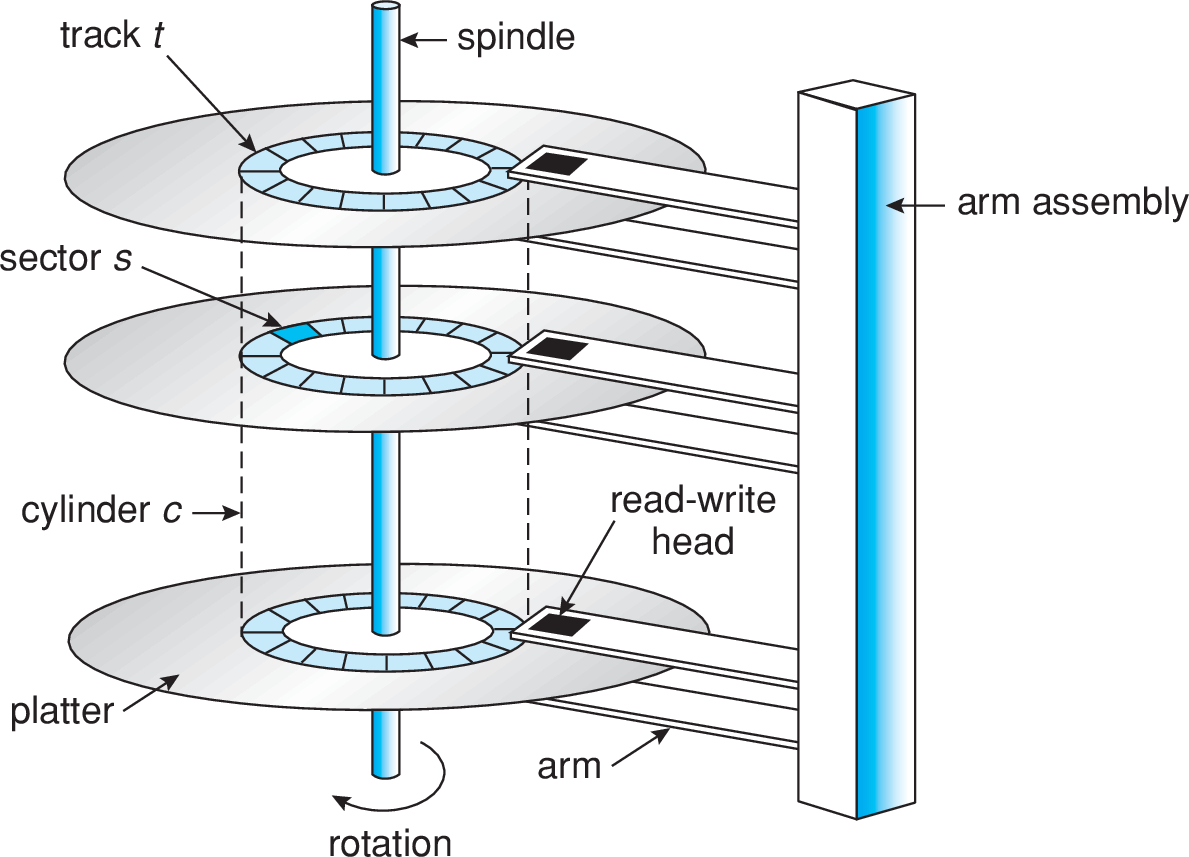
\includegraphics[width=5cm]{figs/03-10_01.pdf}
      \end{center}
    \end{column}
  \end{columns}

\end{frame}

%---------------------------------------------------------------------
\begin{frame}
  \frametitle{Discos magnéticos}
  
  Lo que importa es la {\bf tasa de transferencia} de datos entre
  disco y memoria principal.

  {\bf Tiempo de posicionamiento} o ``tiempo de acceso aleatorio''
  depende de:
  \begin{itemize}
    \item {\bf Seek time}, tiempo de búsqueda, para mover el brazo hasta el cilindro buscado
    \item {\bf Latencia rotacional}, tiempo necesario para que el sector buscado quede debajo del brazo
    \item Ambos del orden de {\em msec}
  \end{itemize}
  Tasas de transferencia pueden llegar a los MB/{\em sec}
  
  \begin{itemize}
    \item {\bf Host controller} es parte del sistema computacional
    \item {\bf Disk controller} es parte del disco
    \item S.O. hace solicitudes al {\bf host controller}, el cual envía comandos al {\bf device controller}
  \end{itemize}

\end{frame}
%---------------------------------------------------------------------
\begin{frame}
  \frametitle{Discos de Estado Sólido (SSD)}

  \begin{itemize}
    \item Sin {\bf seek time} ni {\bf latencia rotacional}
    \item Más rápidos
    \item Más costoso por MB
    \item Menor consumo eléctrico
  \end{itemize}
\end{frame}

%---------------------------------------------------------------------
\begin{frame}
  \frametitle{Organización}

  Discos están organizados como un arreglo de {\bf bloques lógicos}
  \begin{itemize}
    \item Bloques lógicos típicamente de 512 bytes
    \item Bloques lógicos se mapean a sectores
    \item Sector 0 es el primer sector del primer {\em track} del cilindro más externo
  \end{itemize}

  Conocienco número de platos, {\em tracks} (cilindros $\sim m \times 10^4$ y {\em sectores} ($\sim n \times 10^2$) es posible traducir
  bloque lógico a $\langle \mathit{plato}, \mathit{track}, \mathit{sector} \rangle$
  \begin{itemize}
    \item Aún hay que considerar densidad de sectores
    \item Sectores de cilindros externos {\em pueden} tener más densidad que en sectores internos
  \end{itemize}

\end{frame}

%---------------------------------------------------------------------
\begin{frame}
  \frametitle{Formatos de disco}

  Disco no es más que un conjunto de material magnético
  
  \begin{itemize}
    \item {\bf Formateo de bajo nivel} o {\bf formateo físico}: crea estructura de sectores
      \begin{itemize}
        \item Sector: header + data + trailer (incluyendo ECC)
        \item ECC: Error-Correcting Code, calculado a partir de {\em data}
      \end{itemize}
    \item {\bf Particionamiento}: agrupación de cilindros que son tratados como discos separados
      \begin{itemize}
        \item Tabla de particiones accesible desde un {\bf Master Boot Record} en el primer sector
        \item Típicamente: 4 particiones primarias, o 3 primarias + 1 extendida
        \item Particiones contienen tipos de sistema de archivo
      \end{itemize}
    \item {\bf Formateo lógico}: estructuras para {\em sistema de archivos}
  \end{itemize}

\end{frame}
%---------------------------------------------------------------------
\subsection{{\em Scheduling de accesos}}

\begin{frame}
  \frametitle{Estructura de solicitudes de acceso}

  S.O. efectúa solicitud indicando:
  \begin{itemize}
    \item Lectura o escritura
    \item Dirección de disco
    \item Dirección de memoria (física)
    \item Número de sectores a transferir
  \end{itemize}
  
  Solicitudes son encoladas. 
  \begin{itemize}
    \item El orden en que son atendidas determina la latencia efectiva del controlador de disco
  \end{itemize}
\end{frame}
%---------------------------------------------------------------------
\begin{frame}
  \frametitle{{\em Scheduling} FCFS}
  \framesubtitle{Una vez más, {\em First Come, First Served}}
  
  Justo, pero no necesariamente el de mejor servicio
  
  \begin{center}
    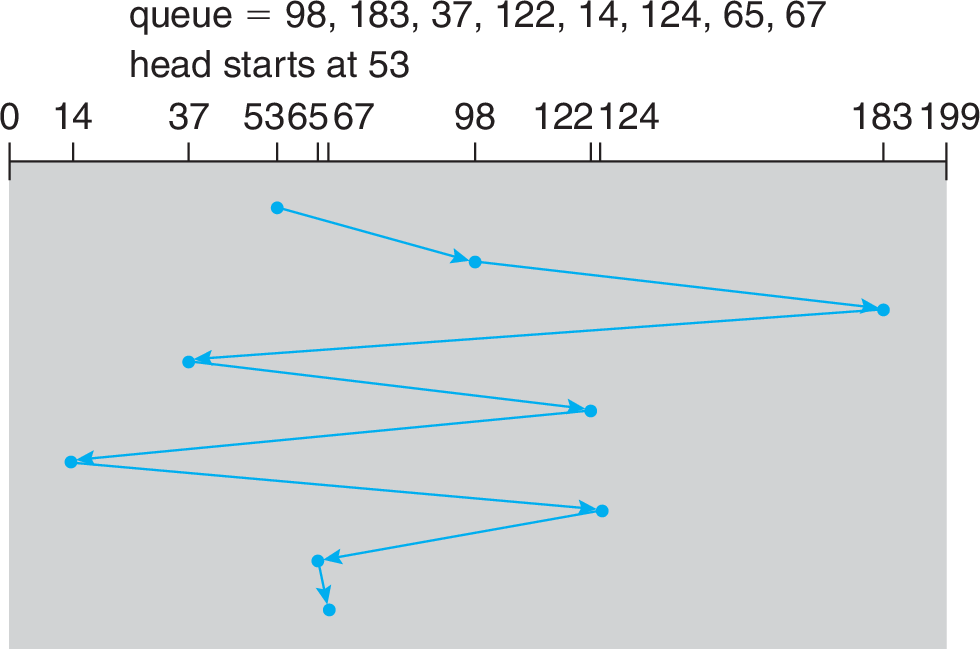
\includegraphics[width=7cm]{figs/03-10_04.pdf}
  \end{center}

  Medida de latencia: desplazamiento que debe hacer el brazo \onslide<2->{$=640$}
  
\end{frame}
%---------------------------------------------------------------------
\begin{frame}
  \frametitle{{\em Scheduling} SSTF}
  \framesubtitle{{\em Shortest Seek Time First}}

  Busca el que esté más cerca de la posición actual

  \begin{center}
    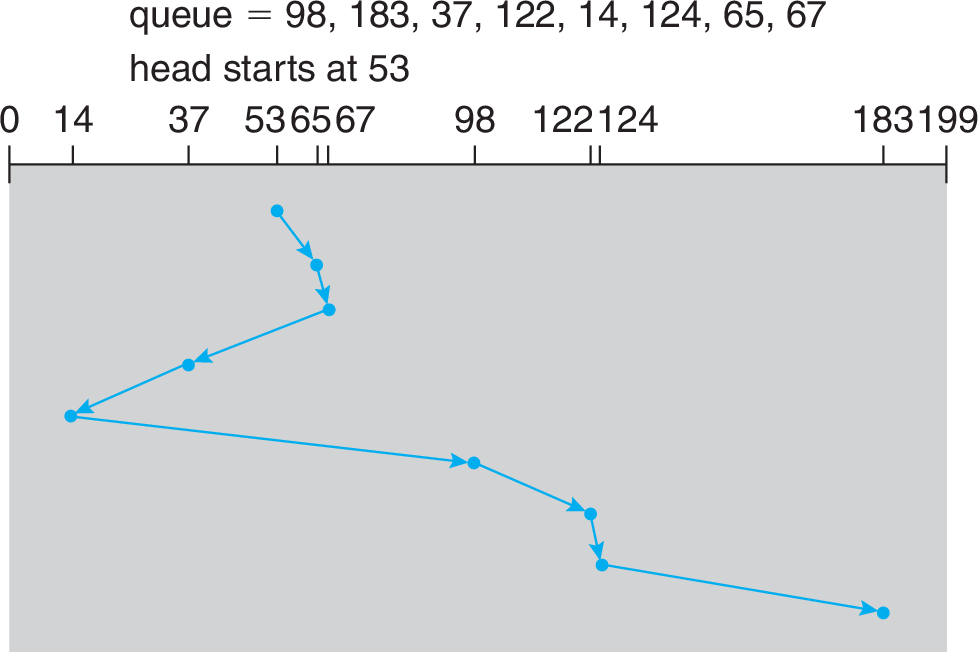
\includegraphics[width=7cm]{figs/03-10_05.pdf}
  \end{center}

  Desplazamiento \onslide<2->{$=208$}
  
  \onslide<3->{{\bf No es óptimo} (¿por qué?)}
\end{frame}
%---------------------------------------------------------------------
\begin{frame}
  \frametitle{{\em Scheduling} SCAN}
  \framesubtitle{a.k.a. el {\em elevador}}

  Brazo se mueve de un extremo a otro y sirve todo lo que encuentre en el camino \ldots
  \onslide<2->{como un ascensor}
  
  \begin{center}
    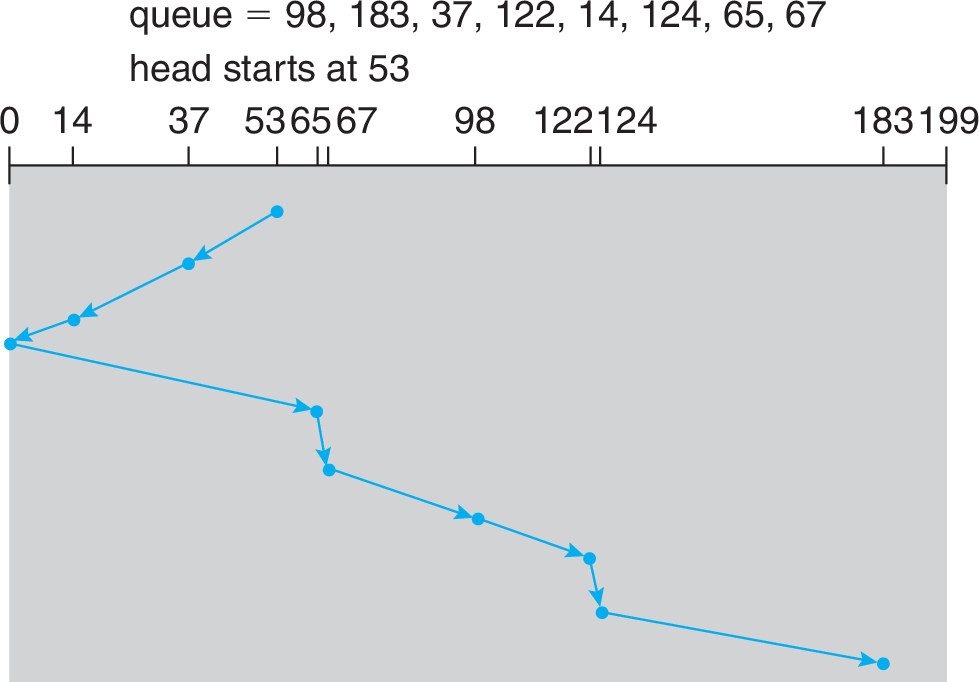
\includegraphics[width=7cm]{figs/03-10_06.pdf}
  \end{center}

  %Desplazamiento \onslide<3->{$=$}
\end{frame}
%---------------------------------------------------------------------
\begin{frame}
  \frametitle{{\em Scheduling} C-SCAN}
  \framesubtitle{a.k.a. el {\em elevador circular} }

  Las solicitudes que llegan justo después que el brazo ha pasado
  ``llevan más tiempo esperando''
  
  Brazo llega a un extremo y se mueve completamente al extremo opuesto, para continuar en el mismo sentido
  \ldots \onslide<2->{como un ascensor circular}
  
  \begin{center}
    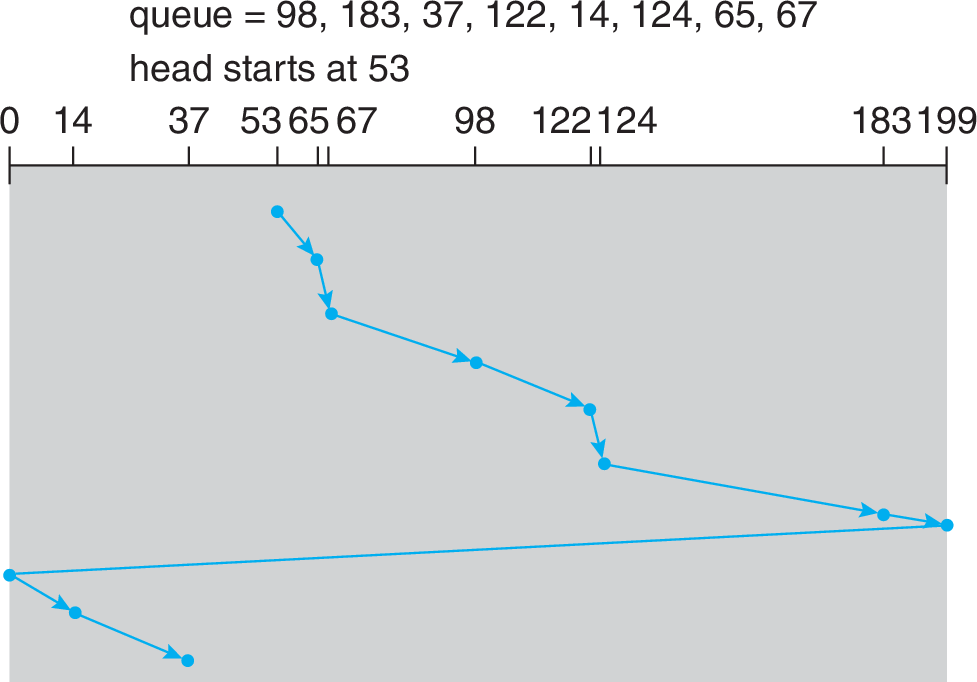
\includegraphics[width=7cm]{figs/03-10_07.pdf}
  \end{center}

  Objetivo es disminuir el tiempo de espera de cada solicitud
  %Desplazamiento \onslide<3->{$=$}
\end{frame}

%---------------------------------------------------------------------
\begin{frame}
  \frametitle{{\em Scheduling} LOOK y C-LOOK}

  Similares a SCAN y C-SCAN, pero no se mueven hasta los extremos si no es necesario

  \begin{center}
    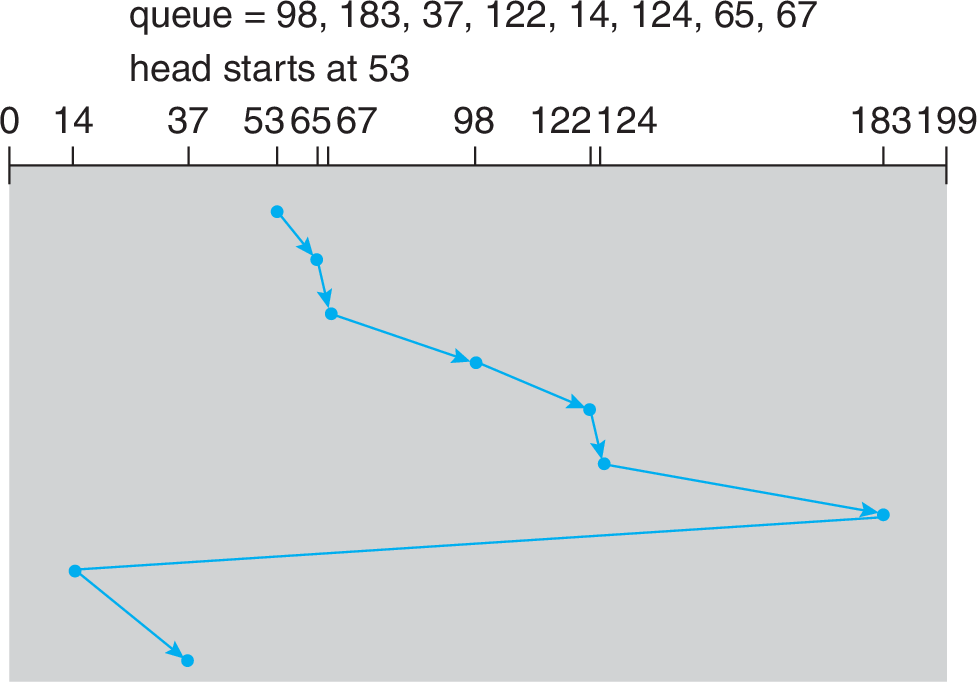
\includegraphics[width=7cm]{figs/03-10_08.pdf}
  \end{center}
  
  
\end{frame}
%---------------------------------------------------------------------
\subsection{RAID}

\begin{frame}
  \frametitle{RAID}
  \framesubtitle{Redundant Array of Independent Disks}
  
  Discos tienen {\em tasas de falla}.
  
  \begin{itemize}
    \item <2->Disco que falla una vez cada $100000$
    \item <3->En un grupo de 100 discos falla uno cada \ldots \onslide<4->{$1000$ horas}
  \end{itemize}
  
  \onslide<5->{Una manera simple de protegerse ante falla es la {\bf redundancia}}
  \begin{itemize}
    \item <6->Estrategia básica de redundancia: {\bf mirroring}
  \end{itemize}
  
\end{frame}

%---------------------------------------------------------------------
\begin{frame}
  \frametitle{RAID}
  \framesubtitle{Redundant Array of Independent Disks}

  Diversas estrategias (niveles) de RAID
  \begin{columns}[c]
    \begin{column}[T]{7cm}
      \begin{itemize}
        \item {\bf RAID 0}: Stripping
        \item {\bf RAID 1}: Mirroring
        \item {\bf RAID 2}: $N$ discos y $N-1$ parity bits
        \item {\bf RAID 3}: $N$ discos $+ 1$ disco de paridad
        \item {\bf RAID 4}: Paridad por bloques
        \item {\bf RAID 5}: Paridad por bloques y distribuida
        \item {\bf RAID 6}: RAID 5 + información adicional para 
                            soportar fallas de dos discos
      \end{itemize}
    \end{column}
    \begin{column}[T]{3.5cm}
      \begin{center}
        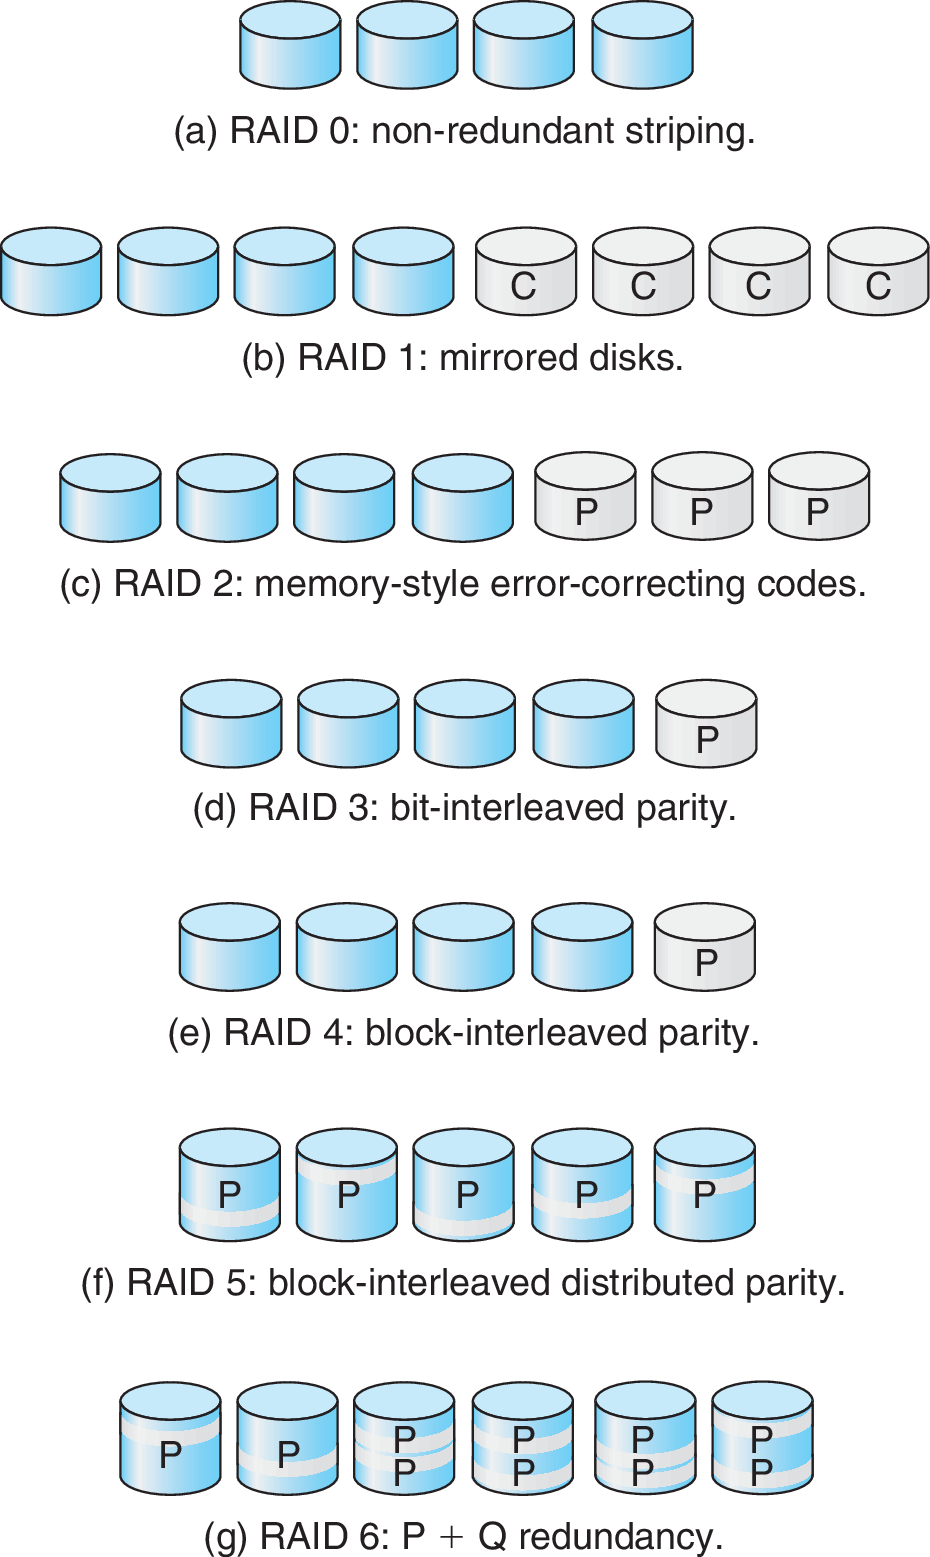
\includegraphics[width=3.5cm]{figs/03-10_11.pdf}
      \end{center}
    \end{column}
  \end{columns}

\end{frame}

%---------------------------------------------------------------------
\begin{frame}
  \frametitle{RAID}
  \framesubtitle{Redundant Array of Independent Disks}

  \begin{columns}[c]
    \begin{column}[T]{7cm}
      \begin{itemize}
        \item {\bf RAID 0+1}: Stripe con mirroring
          \begin{itemize}
            \item Performance de RAID 0
            \item Confiabilidad de RAID 1
            \item Si falla un disco se pierde un {\em stripe}
          \end{itemize}
        \item {\bf RAID 1+0}: Mirror de pares de discos
          \begin{itemize}
            \item Si falla un disco se pierde solo un disco
          \end{itemize}
      \end{itemize}
    \end{column}
    \begin{column}[T]{5cm}
      \begin{center}
        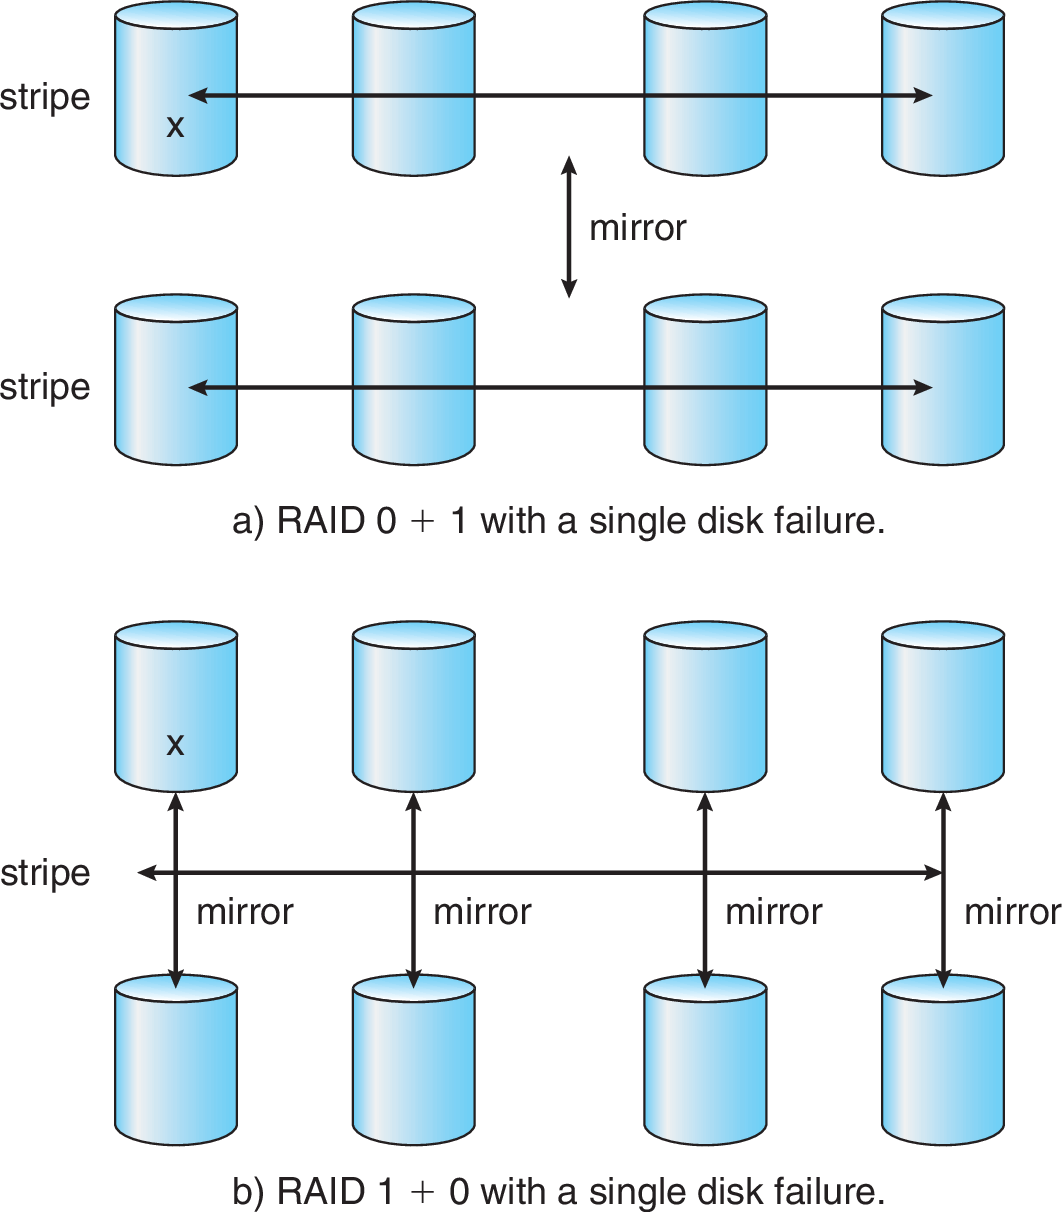
\includegraphics[width=5cm]{figs/03-10_12.pdf}
      \end{center}
    \end{column}
  \end{columns}

\end{frame}

%---------------------------------------------------------------------
\section{Sistemas de Archivos}

\subsection{Archivos}

\begin{frame}
  \frametitle{Archivos}
  
  \begin{block}{{\bf Archivo}}
    Colección de información en almacenamiento secundario  
  \end{block}
  \begin{itemize}
    \item<2->{Unidad mínima de alamcenamiento para el usuario}
    \item<3->{Agrupación lógica de {\em bytes}}
  \end{itemize}
  
  \onslide<4->{Contenido: cualquier cosa}
  \begin{itemize}
    \item<5-> Significado está determinado por la forma en que se utiliza
          su contenido
    \item<5-> Texto, imagen, código fuente, código binario (ejecutable), \ldots
  \end{itemize}
  
\end{frame}
%---------------------------------------------------------------------
\begin{frame}
  \frametitle{Archivos}
  \framesubtitle{Atributos de archivos}
  
  Cómo caracterizar un archivo
  \begin{itemize}
    \item {\bf Nombre} (simbólico). Información {\em human-readable}
    \item {\bf Identificador}. Determinado por el S.O.
    \item {\bf Tipo}.
    \item {\bf Ubicación}. Puntero a dirección de disco.
    \item {\bf Tamaño}. Tamaño actual en {\em bytes}, {\em words} ó {\em blocks}. 
                  Puede incluir un tamaño máximo.
    \item {\bf Proteccion}. Datos de control de acceso. Lecturas, escritura, ejecución.
    \item {\bf Fecha}. Creación, acceso, modificación.
    \item {\bf Usario}. Propietario.
    \item {\bf Atributos extendidos}
      \begin{itemize}
        \item Codificación, {\em checksum}, programas asociados
      \end{itemize}
  \end{itemize}
  Información de archivos de se almacena en la estructura de directorios.
\end{frame}
%---------------------------------------------------------------------
\begin{frame}
  \frametitle{Archivos}
  \framesubtitle{Operaciones sobre archivos}

  S.O. provee {\em syscalls} para ejecutar operaciones sobre archivos
  
  \begin{itemize}
    \item {\bf Creación}
    \item {\bf Escritura}
    \item {\bf Lectura}
    \item {\bf Reposicionamiento}
    \item {\bf Eliminación} (borrar)
    \item {\bf Reducción} (truncar) 
  \end{itemize}
  
\end{frame}

%---------------------------------------------------------------------
\begin{frame}
  \frametitle{Archivos}
  \framesubtitle{Apertura y cierre}

  Acceder un archivo requiere {\bf buscarlo} en una estructura de directorio
  
  \onslide<2->{Para evitar este proceso, se usa una {\bf lista de archivos abiertos}}
  
  \begin{itemize}
    \item<3-> {\tt open()}. Al abrir un archivo se carga en esta lista algunos datos
      \begin{itemize}
        \item Puntero de acceso. Desplazamiento ({\em offset}) desde el inicio del archivo.
        \item Cantidad de aperturas. Contador de cuántas veces se encuentra abierto.
        \item Ubicación en disco.
        \item Permisos de acceso.
      \end{itemize}
    \item<4-> {\tt close()}. Cierra el archivo. Si nadie más lo está ocupando, es eliminado
              de la lista.
  \end{itemize}
  \onslide<5->{S.O. permiten definir {\em locks} de escritura y/o lectura sobre archivos}
\end{frame}

%---------------------------------------------------------------------
\begin{frame}
  \frametitle{Archivos}
  \framesubtitle{Tipos de archivo}

  \begin{columns}[c]
    \begin{column}[T]{7cm}
      \begin{itemize}
        \item Ayudan a determinar qué hacer con el archivo
        \item Ayudan a navegar su estructura
        \item Almacenado como atributo del archivo
        \item \ldots o usando {\em extensiones} en el nombre
          \begin{itemize}
            \item Extensión puede no coincidir con el tipo de archivo
            \item Algunos SS.OO. usan un código identificar en cada archivo:
                {\bf magic number}
          \end{itemize}
      \end{itemize}
    \end{column}

    \begin{column}[T]{5cm}
      \begin{center}
        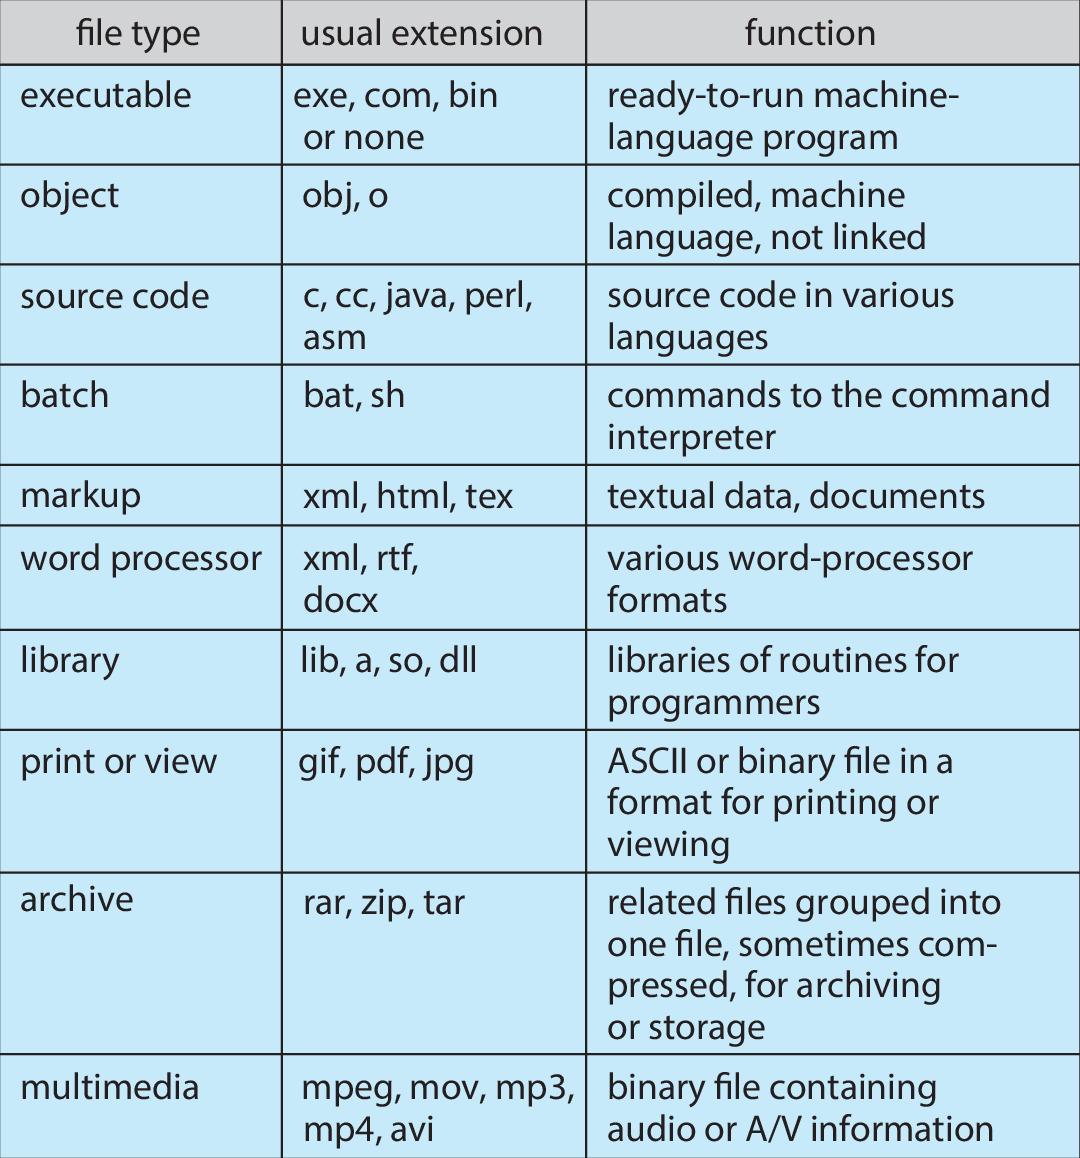
\includegraphics[width=5cm]{figs/03-11_03.pdf}
      \end{center}
    \end{column}
  \end{columns}
  
\end{frame}

%---------------------------------------------------------------------
\begin{frame}
  \frametitle{Archivos}
  \framesubtitle{Acceso a archivos}

  Secuencial \ldots \onslide<2->{o no-secuencial}
  
  \begin{itemize}
    \item Archivos se abren con un {\em puntero} a la próxima ubicación
          que será leída/escrita
    \item Puntero inicializado en $0$
    \item {\bf Acceso Secuencial} permite acceder a una posición a la vez
    \item {\bf Acceso Directo} permite posicionar el puntero en cierta posición del archivo
      \begin{itemize}
        \item ¿Cómo llegar a una posición cualquiera?
        \item La estructura de almacenamiento de archivo debe permitirlo (S.O.)
      \end{itemize}
  \end{itemize}

\end{frame}
%---------------------------------------------------------------------
\subsection{Directorios}

\begin{frame}
  \frametitle{Directorios}

  ¿Cómo encontrar archivos?
  
  \begin{itemize}
    \item Sistemas de archivos mantienen {\em listas} de archivos y sus ubicaciones
          en bloques de disco
    \item Archivos se listan en una {\bf tabla de contenidos} ó {\bf directorio}
  \end{itemize}
  
  Operaciones importantes
  \begin{itemize}
    \item Buscar un archivo: {\tt find}, {\tt grep}, {\tt locate}
    \item Agregar un archivo a directorio: {\tt mv}, {\tt cp}, {\tt move}, {\tt copy}
    \item Eliminar un archivo del directorio: {\tt rm}, {\tt del}
    \item Listar los archivo en un directorio: {\tt ls}, {\tt dir}
    \item Reubicar un archivo entre directorios: {\tt mv}, {\tt move}
    \item Navegar por los directorios: {\tt cd}
  \end{itemize}
\end{frame}

%---------------------------------------------------------------------
\begin{frame}
  \frametitle{Directorio de uno y dos niveles ({\em single-level} y {\em two-level)}}

  Todos en el mismo directorio
  \begin{center}
    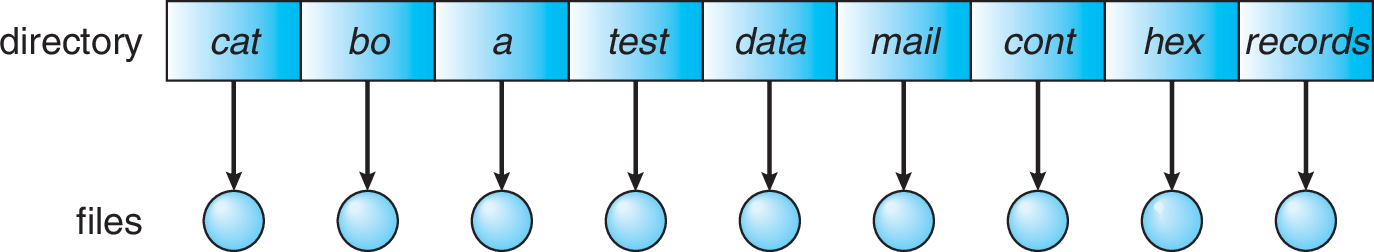
\includegraphics[width=8cm]{figs/03-11_09.pdf}
  \end{center}

  Un directorio por usuario
  \begin{center}
    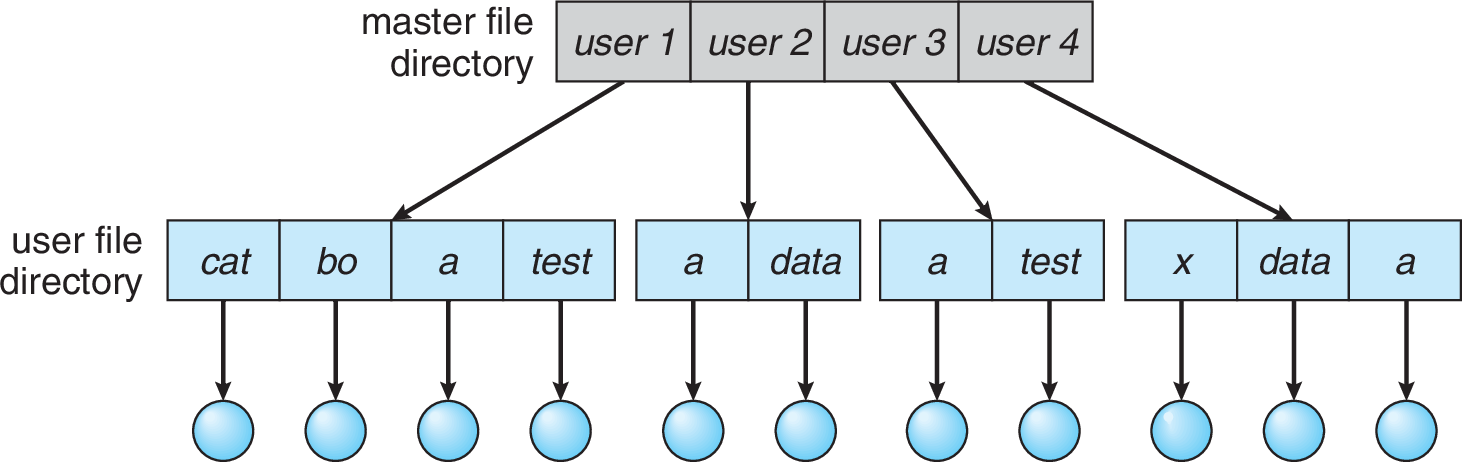
\includegraphics[width=8cm]{figs/03-11_10.pdf}
  \end{center}

\end{frame}
%---------------------------------------------------------------------
\begin{frame}
  \frametitle{Árboles de directorios}

  \begin{itemize}
    %\item Entradas en un directorio pueden ser archivos o directorios
    \item Camino desde la raíz al directorio: {\bf ruta} ó {\bf path}
    \item Cada proceso tiene un directorio actual: {\bf current directory} ({\tt pwd})
    \item {\bf Ruta absoluta}: Ruta desde la raíz. Ej: {\tt /spell/mail/exp}
    \item {\bf Ruta relativa}: Ruta desde la ubicación actual ({\em current directory}).
          Ej: {\tt p/list} solo existe si el directorio actual es {\tt /programs/}
  \end{itemize}

  \begin{center}
    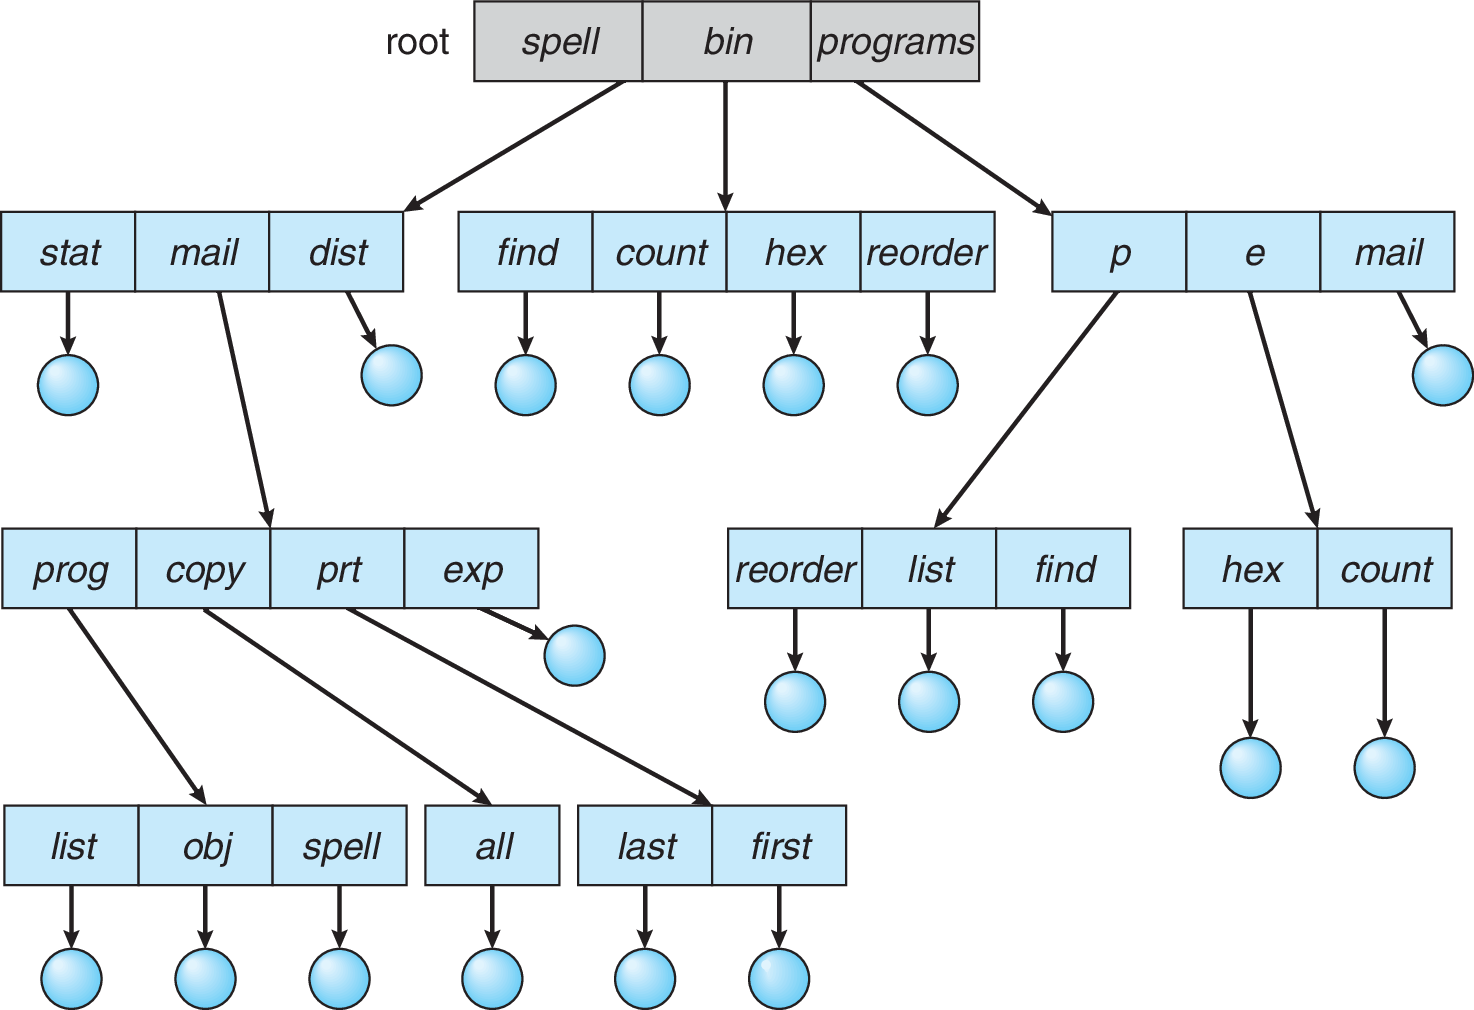
\includegraphics[width=7cm]{figs/03-11_11.pdf}
  \end{center}


\end{frame}

%---------------------------------------------------------------------
\begin{frame}
  \frametitle{Directorios como grafos acíclicos}

  Una manera sencilla de compartir archivos: que el mismo archivo pertenezca a dos directorios
  \begin{center}
    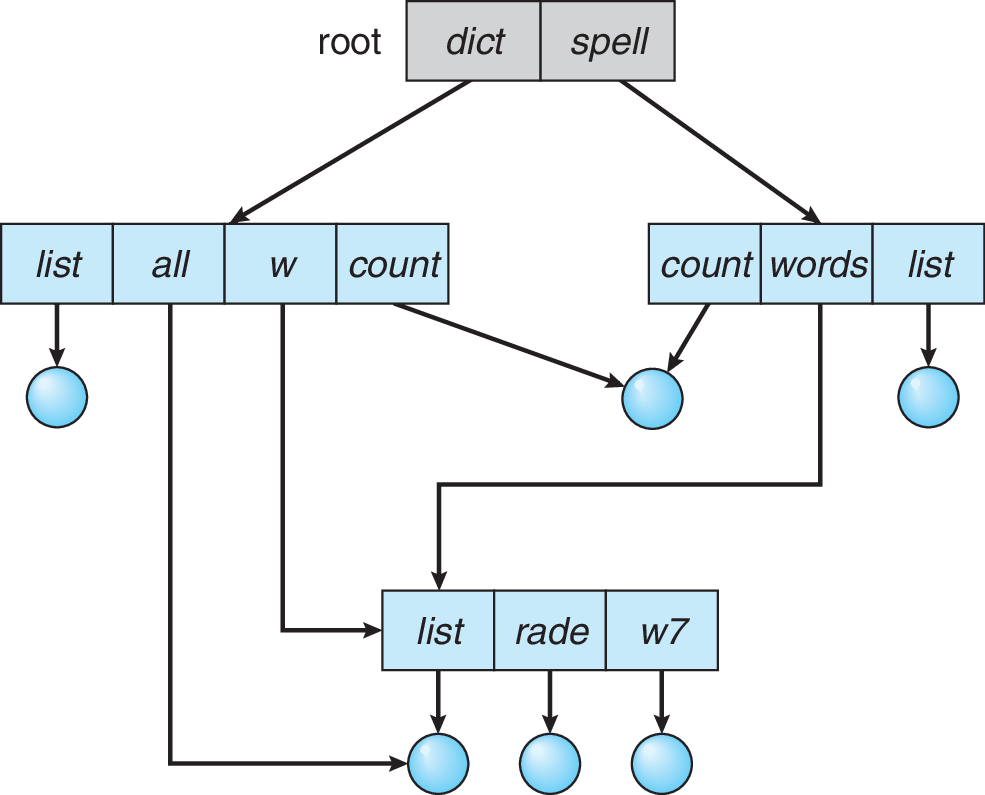
\includegraphics[width=5cm]{figs/03-11_12.pdf}
  \end{center}
  \begin{itemize}
    \item Implementación usando {\bf link}s
      \begin{itemize}
        \item {\bf Symbolic links}: {\em link} a nombre de archivo ({\tt ln -s})
        \item {\bf Hard link}: {\em link} a archivo ({\tt ln})
      \end{itemize}
    \item ¿Cómo recorrer el directorio?
  \end{itemize}
  
\end{frame}
%---------------------------------------------------------------------
\begin{frame}
  \frametitle{Directorios como grafos acíclicos}

  ¿Qué hacer al borrar un archivo?
  \begin{itemize}
    \item {\bf Symbolic links}. Si se borra el archivo original, el {\em link}
          sigue existiendo, y debe ser eliminado manualmente
          \begin{center}
            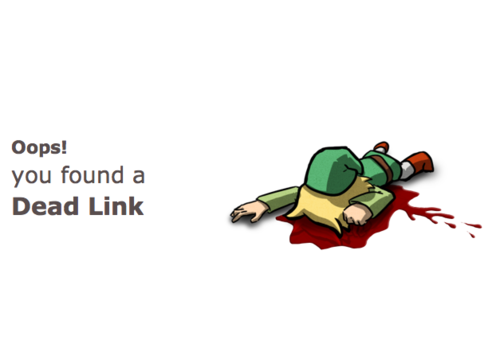
\includegraphics[width=6cm]{figs/03-deadlink.png}
          \end{center}
    \item {\bf Hard links}. {\em Links} aumentan un contador de referencias el archivo.
          El archivo solo es eliminado cuando no quedan más referencias a él.
  \end{itemize}

\end{frame}
%---------------------------------------------------------------------
\begin{frame}
  \frametitle{Montaje de sistemas de archivos}

  Para acceder a sistemas de archivos se necesita un {\em punto de acceso},
  que asigna una posición de directorio a bloques de disco (por ejemplo, particiones)
  \begin{itemize}
    \item Operación {\tt mount} hace que un sistema de archivos sea accesible desde un lugar
          conocido, como {\bf mount point}
    \item Ejecución: {\tt mount /users /device/disk2}
  \end{itemize}

  \begin{center}
    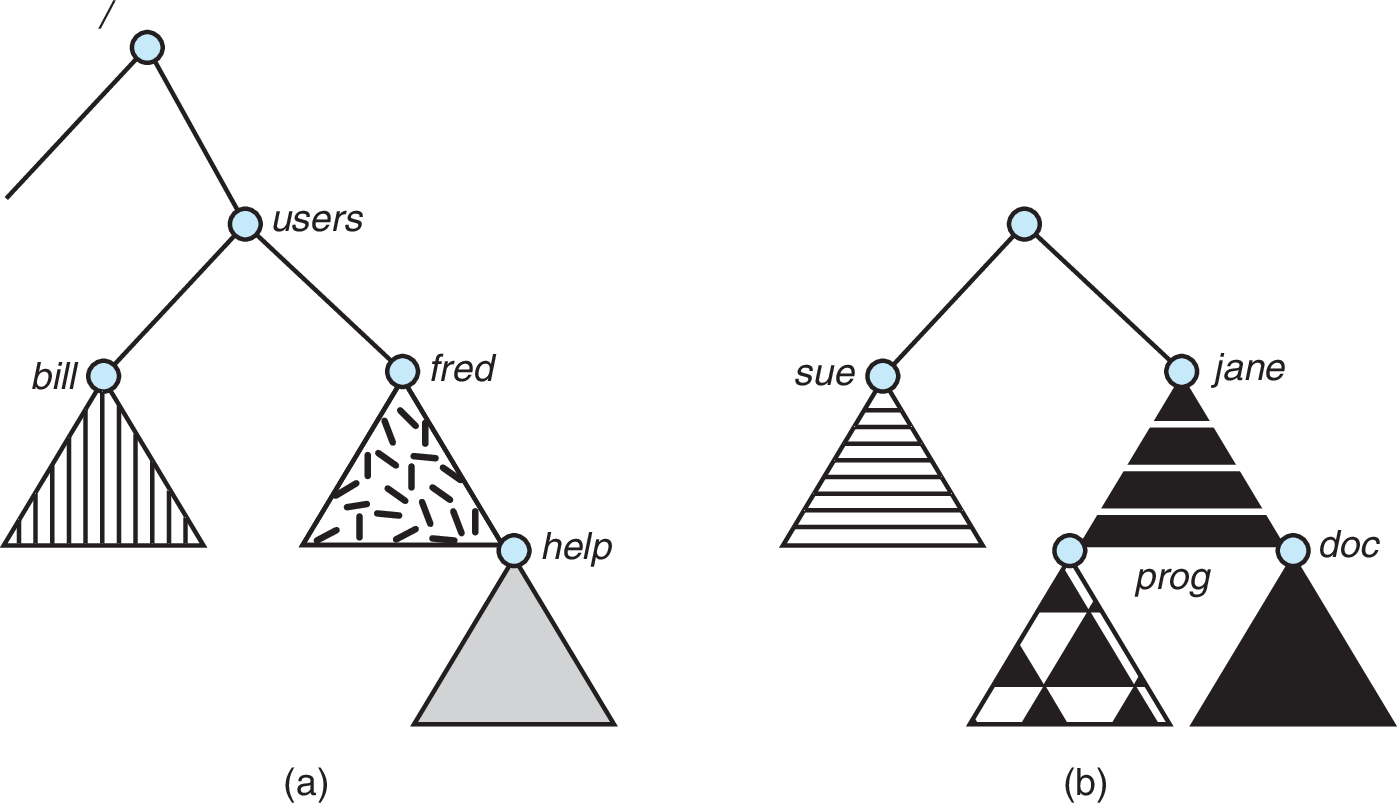
\includegraphics[width=6cm]{figs/03-11_14.pdf}
    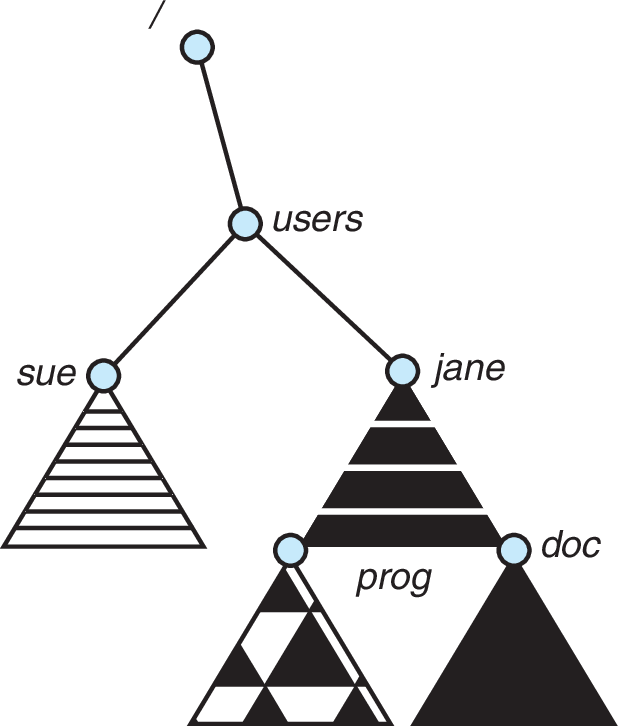
\includegraphics[width=3cm]{figs/03-11_15.pdf}
  \end{center}

\end{frame}
%---------------------------------------------------------------------
\subsection{Implementación de Sistema de Archivos}

\begin{frame}
  \frametitle{Sistemas de archivos}

  Un {\bf sistema de archivos} permite obtener una dirección de disco,
  a partir de un datos simbólicos: nombre de archivo, directorio, rutas, links, \ldots
  
  Algunos ejemplos:
  \begin{itemize}
    \item ISO9660 (CD-ROMs)
    \item UFS: Unix File System, basado Berkeley Fast File System (FFS)
    \item FAT, FAT32, NTFS: Windows
    \item ext3, ext4: Linux
    \item GFS, FUSE
  \end{itemize}

\end{frame}

%---------------------------------------------------------------------
\begin{frame}
  \frametitle{Sistemas de archivos}

  Elementos típicos de un sistema de archivos:
  \begin{itemize}
    \item {\bf Boot Control Block}. Uno por volumen. Permite utilizar el sistema de archivo para arranque.
      \begin{itemize}
        \item Unix: Boot block
        \item Windows: Partition Boot Sector
      \end{itemize}
    \item {\bf Volume Control Block}. Contiene datos de formato de la partición.
      \begin{itemize}
        \item Unix: Superblock
        \item Windows: Master File Table
      \end{itemize}
    \item Estructura de {\bf directorio}. Ubicaciones de archivos.
    \item {\bf File Control Block}. Uno por archivo. Contiene atributos de archivo.
  \end{itemize}

  \begin{center}
    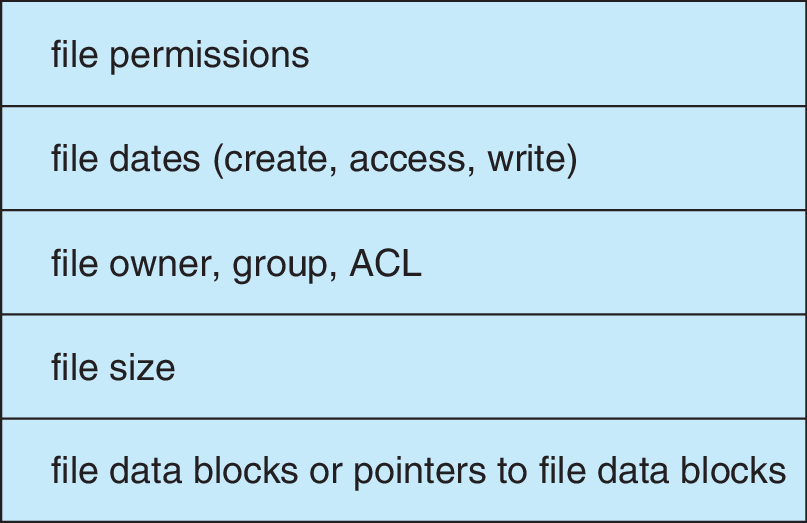
\includegraphics[width=4cm]{figs/03-12_02.pdf}
  \end{center}

\end{frame}
%---------------------------------------------------------------------
\begin{frame}
  \frametitle{Sistemas de archivos}
  Estructuras en memoria principal:
  \begin{itemize}
    \item {\bf Mount table}. Tabla de sistema de archivos montados.
    \item Directorios recientes
    \item Tabla de archivos abiertos en el sistema
    \item Tabla de archivos abiertos por proceso
    \item Buffers de bloques de disco
  \end{itemize}
  
  \begin{center}
    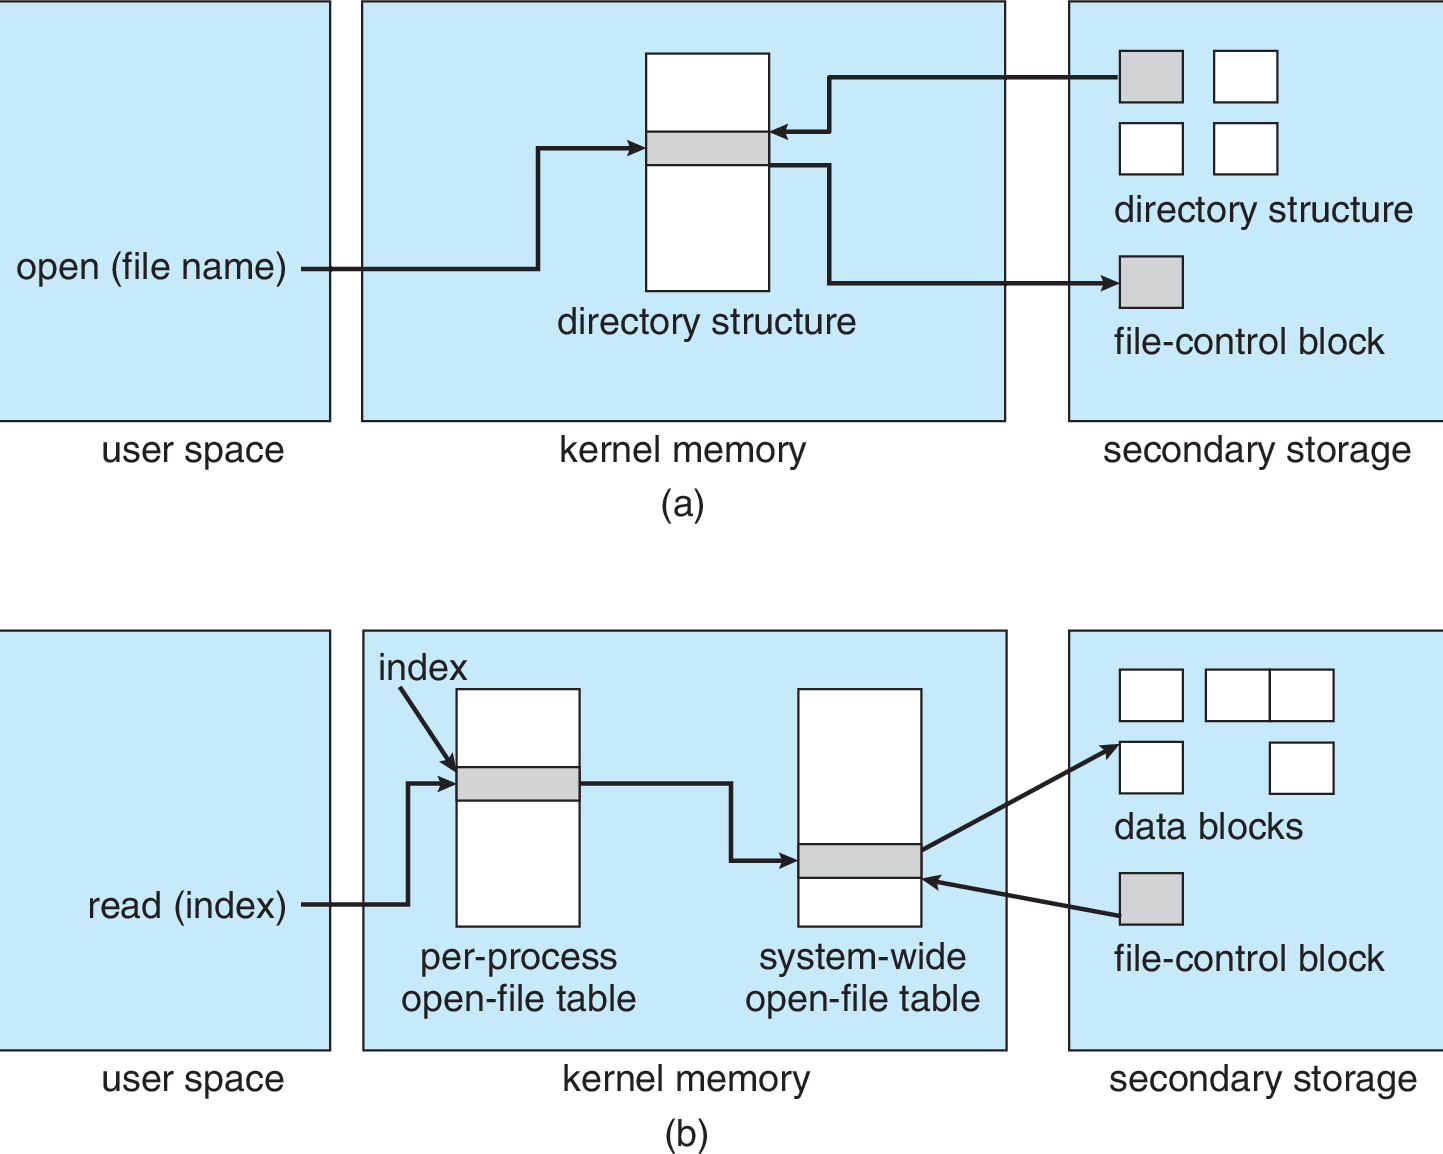
\includegraphics[width=6cm]{figs/03-12_03.pdf}
  \end{center}

\end{frame}

%---------------------------------------------------------------------
\begin{frame}
  \frametitle{Asignación de bloques}

  Cada archivo requiere utilizar bloques de disco
  
  \begin{itemize}
    \item Bloques deben ser asignados de manera eficiente
    \item Mala asignación provocará demoras en tiempos de acceso
    \item Estrategias de asignación de bloques
  \end{itemize}

\end{frame}
%---------------------------------------------------------------------
\begin{frame}
  \frametitle{Asignación de bloques}
  \framesubtitle{Asignación contigua}
  
  \begin{columns}[c]
    \begin{column}[T]{6cm}
      \begin{itemize}
        \item Archivo de $n$ bloques, bloque inicial $b$
        \item Bloques: $b, b+1, \ldots b+n-1$
        \item Fácil de acceder a siguiente bloque
        \item <2-> -Problema: fragmentación externa
        \item <3-> -Require operaciones de {\bf compactación}
              (defragmentación)
      \end{itemize}
    \end{column}
    \begin{column}[T]{5cm}
      \begin{center}
        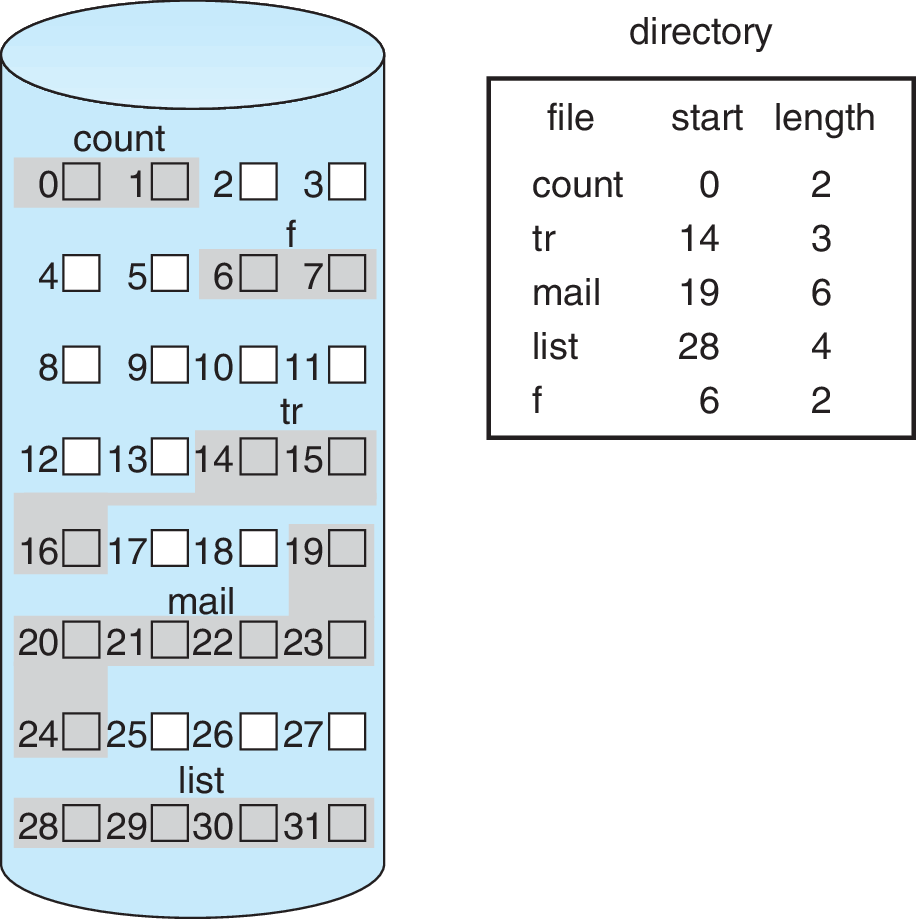
\includegraphics[width=5cm]{figs/03-12_05.pdf}
      \end{center}
    \end{column}
  \end{columns}  
\end{frame}

%---------------------------------------------------------------------
\begin{frame}
  \frametitle{Asignación de bloques}
  \framesubtitle{Asignación enlazada ({\em linked})}

  \begin{columns}[c]
    \begin{column}[T]{6cm}
      \begin{itemize}
        \item Almacena punteros
              a bloque siguiente
        \item Ej: bloque de 512 bytes, solo puede guardar 508 bytes
        \item No requiere tamaño inicial de archivo. Puede crecer.
        \item <2-> -Acceso solo secuencial
        \item <3-> -Se pierde espacio en punteros
        \item <4-> Alternativa: almacenar {\em clusters} de bloques en lugar
                   de bloques individuales (fragmentación interna)
        \item <5-> Vulnerable a falla de un bloque
      \end{itemize}
    \end{column}
    \begin{column}[T]{5cm}
      \begin{center}
        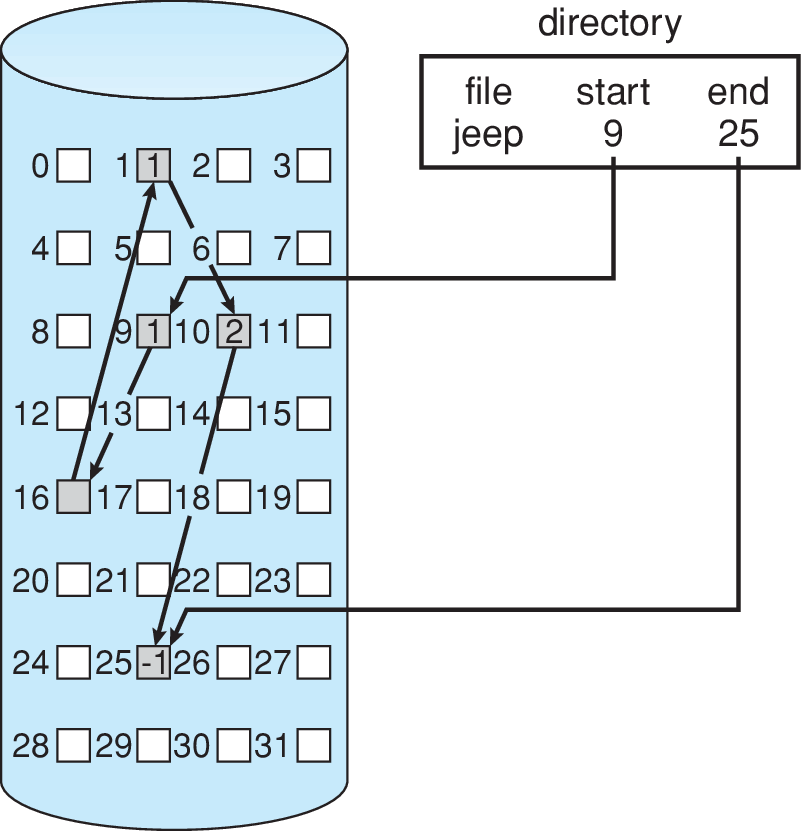
\includegraphics[width=5cm]{figs/03-12_06.pdf}
      \end{center}
    \end{column}
  \end{columns}  
  
\end{frame}
%---------------------------------------------------------------------
\begin{frame}
  \frametitle{Asignación de bloques}
  \framesubtitle{Asignación enlazada ({\em linked}): FAT}

  \begin{columns}[c]
    \begin{column}[T]{6cm}
      \begin{itemize}
        \item FAT: {\bf File Allocation Table}
        \item Tabla al inicio del disco con una entrada por archivo
        \item Último cluster almacena EOF ({\em end-of-file})
        \item <2-> +Mejor acceso aleatorio
        \item <3-> -Limitado por tamaño de tabla (para FAT32, 4GB por archivo)
      \end{itemize}
    \end{column}
    \begin{column}[T]{5cm}
      \begin{center}
        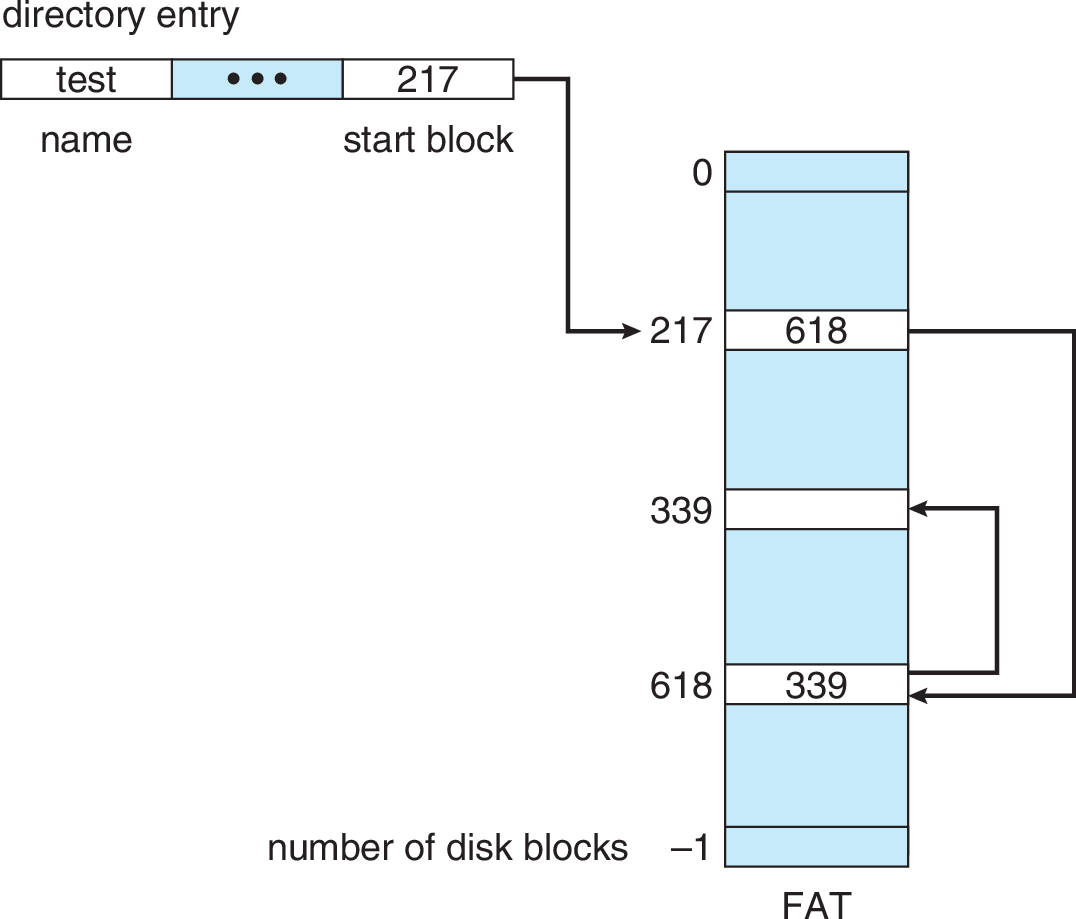
\includegraphics[width=5cm]{figs/03-12_07.pdf}
      \end{center}
    \end{column}
  \end{columns}  
  
\end{frame}

%---------------------------------------------------------------------
\begin{frame}
  \frametitle{Asignación de bloques}
  \framesubtitle{Asignación indexada}

  \begin{columns}[c]
    \begin{column}[T]{6cm}
      \begin{itemize}
        \item Archivos contienen {\em index block}
        \item {\em Index Block} contiene bloques del archivo
        \item Último cluster almacena EOF ({\em end-of-file})
        \item <2-> +Acceso aleatorio sin frag. externa
        \item <3-> -Se pierde espacio por tamaño de {\em index block}
      \end{itemize}
    \end{column}
    \begin{column}[T]{5cm}
      \begin{center}
        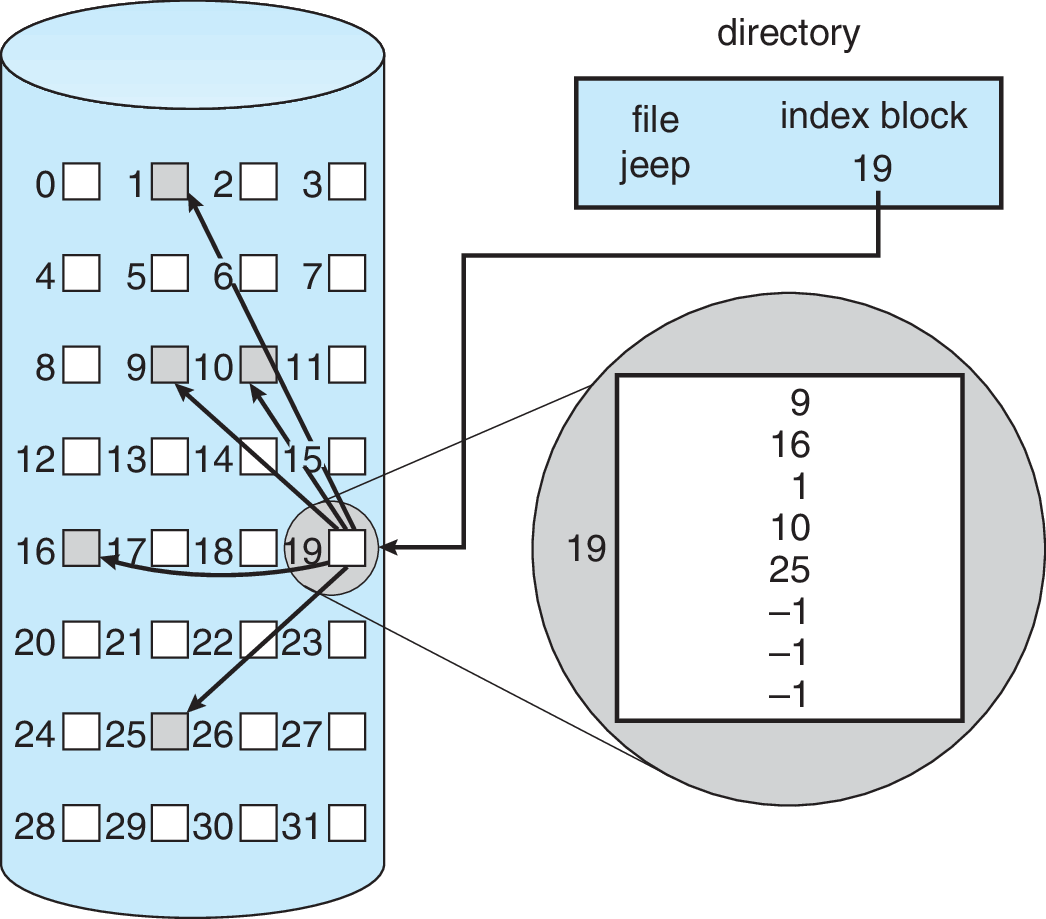
\includegraphics[width=5cm]{figs/03-12_08.pdf}
      \end{center}
    \end{column}
  \end{columns}  

\end{frame}
%---------------------------------------------------------------------
\begin{frame}
  \frametitle{Asignación de bloques}
  \framesubtitle{Asignación indexada: tamaño del {\em index block}}

  \begin{columns}[c]
    \begin{column}[T]{6cm}
      \begin{itemize}
        \item {\bf Esquema enlazado}: última entrada de {\em index block} apunta a otro {\em index block}
        \item {\bf Índice multinivel}: similar a tablas de página multinivel
          \begin{itemize}
            \item Ej: blocks de 4KB, permiten 1024 punteros (de 32-bit)
            \item Dos niveles permiten direccionar $1048576$ bloques $\to 4$GB
          \end{itemize}
        \item {\bf Esquema combinado}: primeros $p$ punteros son bloques directos,
              los siguientes apunta bloque de índice simple, los siguientes a bloque 
              de índice doble, etc
      \end{itemize}
    \end{column}
    \begin{column}[T]{5cm}
      \begin{center}
        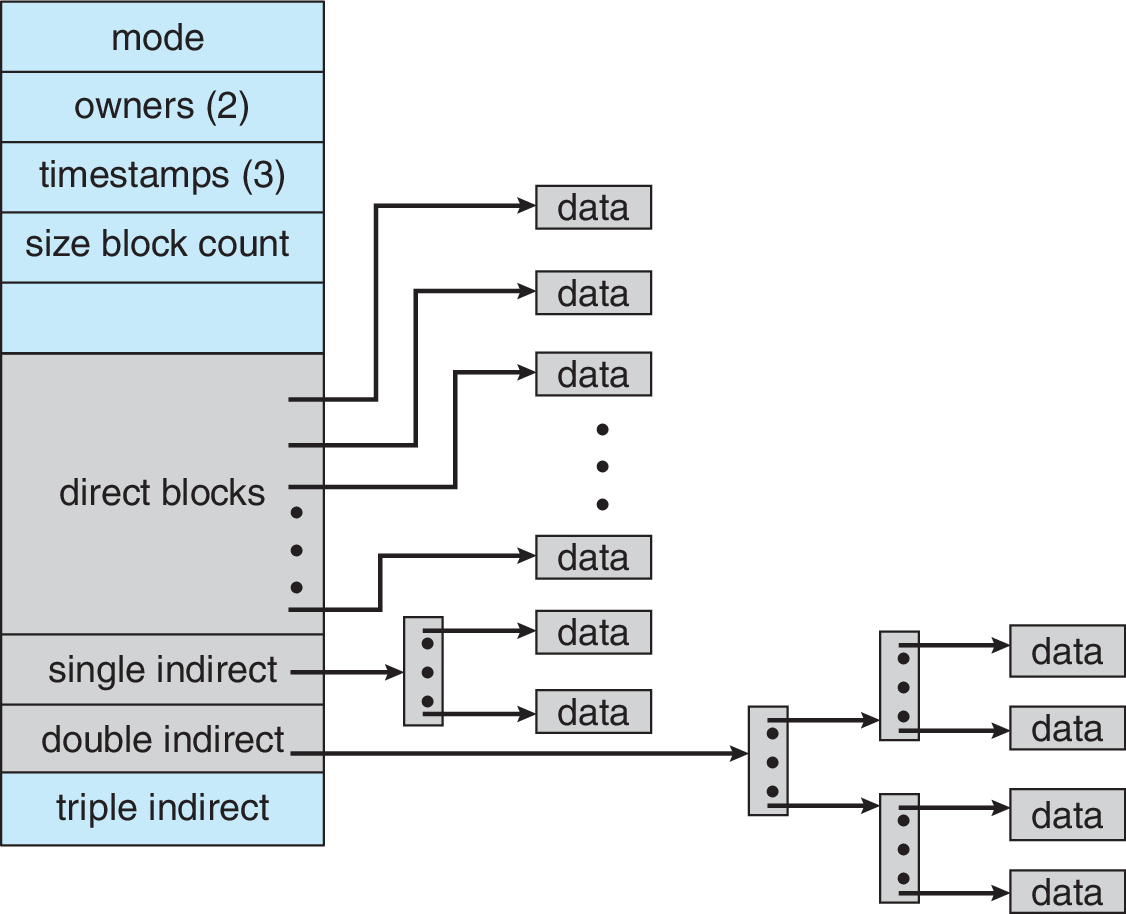
\includegraphics[width=5cm]{figs/03-12_09.pdf}
      \end{center}
    \end{column}
  \end{columns}  

\end{frame}

%---------------------------------------------------------------------
\begin{frame}
  \frametitle{Espacio libre}
  \framesubtitle{¿Cómo encontrarlo?}

  {\bf Bit vector} ó {\bf bitmap} de bloques libres
  
  \begin{itemize}
    \item +Sencillo, eficiente, e implementable en {\em hardware}
    \item -No escala tan bien
      \begin{itemize}
        \item Disco de 1.3GB, con bloques de 512 byte $\to 332$KB
        \item Disco de 1TB, con bloques de 4KB $\to 256$MB 
      \end{itemize}
  \end{itemize}
\end{frame}

%---------------------------------------------------------------------
\begin{frame}
  \frametitle{Espacio libre}

  \begin{columns}[c]
    \begin{column}[T]{6cm}
      {\bf Lista enlazada}
        \begin{itemize}
          \item Punteros a bloques libres
          \item Bloques nuevos se agregan a la lista
          \item -Poco eficiente
          \item <2-> Mejora: agrupar espacios contiguos
          \item <3-> Mantener punteros a espacios libres + número de espacios contiguos
        \end{itemize}
    \end{column}
    \begin{column}[T]{6cm}
      \begin{center}
        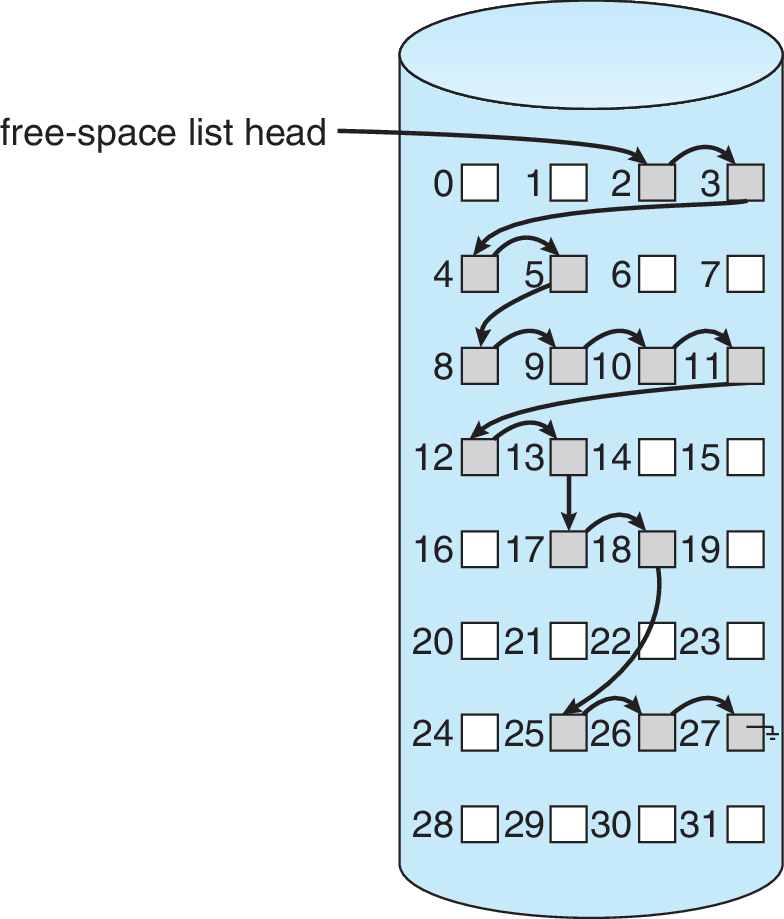
\includegraphics[width=5cm]{figs/03-12_10.pdf}
      \end{center}
    \end{column}
  \end{columns}
\end{frame}
%---------------------------------------------------------------------
%\section{Sistemas de Entrada y Salida}


%---------------------------------------------------------------------
\end{document}